\documentclass{task_description}

\usepackage{xcolor}
\usepackage{pdfpages} 
\newcommand\notes[1]{\textcolor{red}{#1}}

\begin{document}

\thispagestyle{firstpage}
\vspace*{23mm}%
\hfill\parbox[t]{65mm}{

Timothy Zemp\\
Hagenholzstrasse 92\\
8052 Z\"urich\\[5mm]
Matrikel-Nr. 13-915-632\\
timothy.zemp@uzh.ch\\[15mm]
July 27, 2020 \\
}
\vspace*{5mm}
\subsection*{Master's Thesis Specification}

\section*{Separating Wheat From Chaff: Detecting Genuine Continuous Integration Configurations}

Continuous Integration (CI) is a software development practice introduced by the Agile movement with the aim of delivering reliable software releases fast~\cite{Humble:2010}.
Whenever a change is pushed to a remote software repository (\eg GitHub), a build server tool (\eg Travis-CI) detects this change and triggers the integration pipeline.
The pipeline typically consists of several steps, \ie compilation, unit testing, packaging, integration testing, installation and deploy and is usually defined within a configuration file (\eg {}.travis-ci.yml in case of Travis CI).
The success of CI has also lead to a spike in empirical research on this topic that investigated the impact of CI on code review or developers.
Studies show that, for example, CI leads to a higher code commitment frequency and reduced code chunks \cite{zhao2017impact}, different programming languages shows different adoption times (\eg Ruby as being an early-adopter, whereas Java projects tend to adopt later)\cite{vasilescu2014continuous}, and proper build configurations should be maintained in order to reduce long build durations\cite{ghaleb2019empirical}.

Many free cloud CI providers exist, like Travis-CI or Jenkins, and they are easy to adopt: once a repository is registered, it is sufficient to maintain a single configuration in the repository to use the service.
Due to this low entrance barrier, many public repositories contain such configuration files.
Naturally, many of them do not use CI seriously though, the developers might have played around with the provider or the repository is a toy-project alltogether.
Unfortunately, many studies do not differentiate between these cases and treat every project with a configuration file as a valid instance (\eg \cite{zhao2017impact}, \cite{vasilescu2014continuous}, \cite{ghaleb2019empirical}), which might dilute the results, which presents a real threat to validity of an empirical studies on CI.

Inspired by Munaiah et al.\cite{munaiah2017curating}, who created Rreaper\footnote{https://github.com/RepoReapers/reaper}, a tool that can detect seriously engineered repositories, we want to do the same for CI configurations and create a tool that can assess the \emph{genuineness} of a pipeline configuration.
To this end, we need to identify various \emph{features} that describe the configuration (e.g., length, complexity, or number of configuration changes), build automated extraction facilities, and train a classifier (e.g., Decision Tree, Random Forst Classifier).
To assess the success of the approach, we will establish a manually investigated \emph{Ground Truth} dataset that can be used in an automated evaluation.

%%%%%%%%%%%%%%%%%%%%%%%%%%%%%%%%%%%%%%%%
\subsection*{Research Goals}

The goal of this master's thesis is to understand how to automatically detect genuine CI configurations, to study the impact of such a classifier, and to make it easy for future studies to avoid this threat of validity.
To reach this goal, it is necessary to answer the following research questions:


\begin{description}
%
\item[RQ1: Why do repositories contain pseudo configuration files?]
First, we analyze the reasons why software projects contain pseudo configurations (\ie in opposite to genuine configurations).
A side effect of this investigation is the creation of a labelled dataset of \emph{genuine} and \emph{pesudo} configuration files.
%
\item[RQ2: Is it possible to automatically detect genuine CI configurations?]
This RQ provides initial proof that the thesis goal is achievable.
We will define an infrastructure that can extract arbitrary CI-related features for existing projects, and use our ground truth dataset to train a classifier and assess its accuracy in a 10-fold cross evalaution.
%
\item[RQ3: What is the predictive value of different feature categories?]
We intend to extract features on three different levels: \emph{configuration-features} can be extracted from the configuration itself (e.g., how many lines?), \emph{repository-features} can be extracted from the containing repository (e.g., how often has the config been changed?), and \emph{CI-features} can be extracted from the CI provider (e.g., how many builds have been performed in this project?). In this RQ, we will analyze whether simple configuration features are sufficient to yield accurate classifications, or whether advanced feature should be taken into consideration.
%
\item[RQ 4: Are \emph{engineered} projects (\emph{reaper}) also \emph{genuine}?]
Previous work has identified \emph{engineered} projects. This does not automatically imply a \emph{genuine} CI configuration, but there might be a relation to uncover. We are interested in understanding how both populations of projects compare and whether it is necessary to have two independent classifiers.
%
\item[RQ 5: What impact does the classifier have on CI-based studies?]
The last RQ presents a quantification for the motivating problem of this thesis.
We will replicate simple statistics taken from other empirical studies and compare the results when created on \emph{genuine} and \emph{pseudo} configurations.
%
\end{description}

\noindent
In addition to the experimental results, this thesis will produce a usable tool that allows future studies to filter out software projects that do not have genuine CI configurations such they can focus on projects with a meaningful CI configuration.





\newpage
\subsection*{Task description}

The main tasks of this thesis are:

\begin{description}
\item[T1] Research on the topic of CI and the different pipeline configuration mechanism
\item[T2] Data Collection of various repositories using CI and labeling them to establish Ground truth
\item[T3] Definition of extracted features (RQ 1)
\item[T4] Development of classifier
\item[T5] Evaluate the classifier using the reference set and statistical methods (RQ 2/3)
\item[T6] Evaluate correlation between \emph{reaper} and the classifier (RQ 4)
\item[T7] Identify existing CI-studies and evaluate the impact of the classifier (RQ 5)
\item[T8] Write a thesis, comprising the points above
\end{description}

\subsection*{Thesis Structure \& Deliverable}

The thesis consists of several parts. First, basic research is required in order to gain an overview of the different pipeline providers and the possibilities of CI. Afterwards, a Ground Truth Dataset (D1) is established by collecting various repositories adopting CI and labelling them accordingly. Using the data set, suitable features will be identified (RQ 1) and implemented in the classifier. Once enough features are implemented, the classifier is implemented using a prediction algorithm. We conclude the implementation by wrapping the classifier with a Docker Container (D2). This allows other research to easy use the classifier and reproduce our work. We then evaluate the classifier internally (RQ 2/3), evaluate the correlation towards \textit{reaper} (RQ 4) and finally observe the impact of the classifier on existing empirical CI-based studies (RQ 5). Lastly, the thesis is concluded with an academic report (D3).
\\\\
A detailed project plan including the milestones is attached to this proposal and can be found on page \pageref{gantt}.

\begin{description}
\item[D1] Ground Truth Dataset
\item[D2] Classifier
\item[D3] Thesis
\end{description}

\subsection*{Provided resources}

The student does not need any specific resources other than the starting literature, which is referenced in this document. A workplace in the s.e.a.l. lab will be at disposal.

\subsection*{General thesis guidelines}

The typical rules of academic work must be followed. In Bernstein \cite{Bernstein:8} describes a number of guidelines which must be followed. At the end of the thesis, a final report has to be written. The report should clearly be organized, following the usual academic report structure, and has to be written in English using our s.e.a.l. \LaTeX-template. As implementing software is also part of this thesis, State-of-the-Art
design, coding, and documentation standards for the software have to be obeyed. The product of the thesis is the Ground Truth Dataset, a working classifier as well as the written report, that summarizes the process of developing the tool and its evaluation.

\subsection*{Advisors:}


\todo{We need to clarify what to write here... I am not an assistant to Harald anymore :)}

\noindent\textbf{Professor}: \\
\noindent Prof. Dr. Harald C. Gall \\
\\
\noindent\textbf{Responsible assistants}: \\
\noindent Dr.-Ing. Sebastian Proksch (TU Delft) \\


\vspace{2em}
\noindent\textbf{Signatures:}

\vspace{3\baselineskip}
\noindent Timothy Zemp\hfill Prof. Dr. Harald C. Gall
\clearpage
\label{gantt}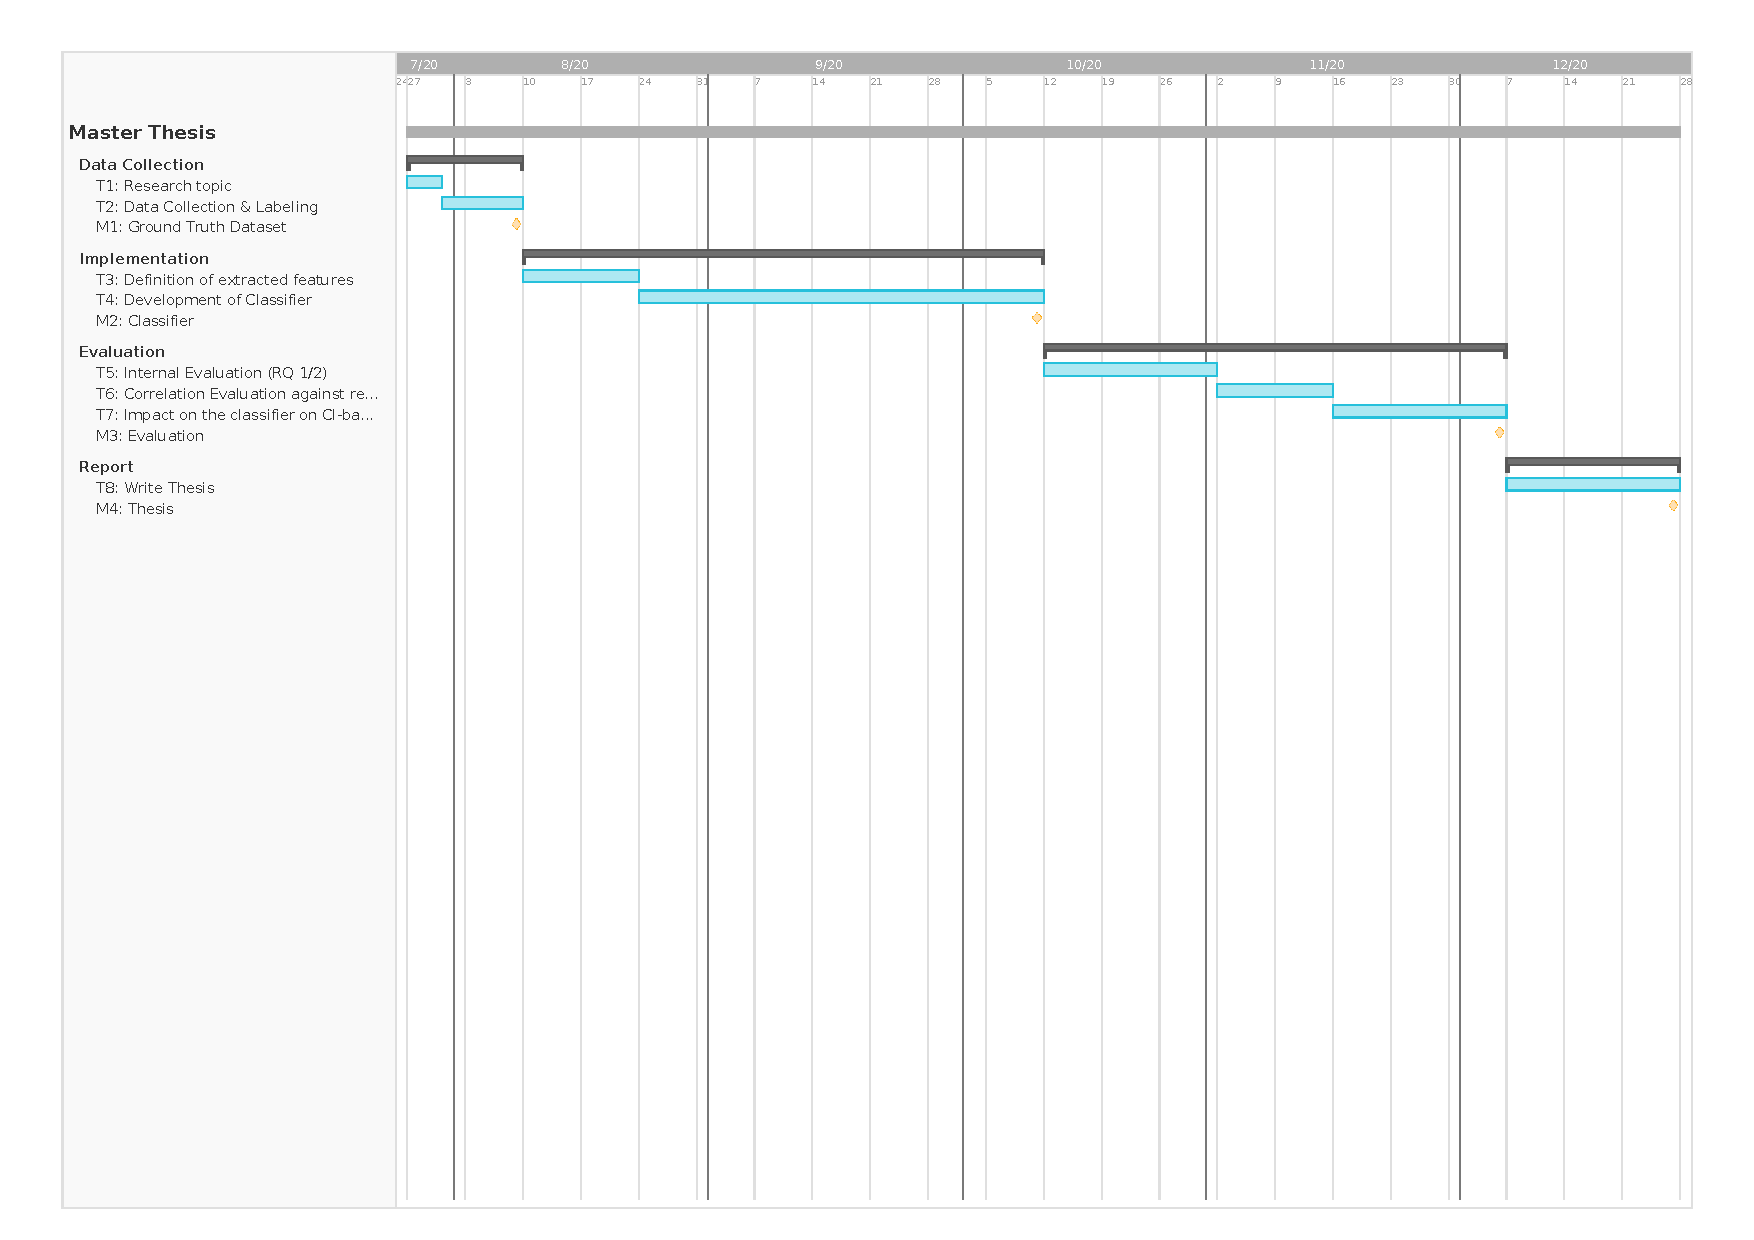
\includepdf[pages={-},fitpaper,rotateoversize]{gantt.pdf}
\bibliographystyle{abbrv}
\bibliography{refs}

\end{document}
